%!TEX root=../document.tex

\section{Einführung}
\label{sec:intro}

Das folgende Dokument befasst sich mit Datamining (auch als knowledge discovery from data oder KDD bekannt). Im heutigen Zeitalter sind wir mit enormen Mengen an Informationen anhand von Daten umgeben. Der Markt produziert weltweit eine gigantische Anzahl an Information bezüglich Finanzgeschichte, Produktbeschreibungen, Performance Logs, Kundenfeedback und vielem mehr. 

Eine Suchmaschine (z.B. Google) erhält hunderte von Anfragen jeden Tag. Jede einzelne dieser Anfragen kann als Transaktion gesehen werden. Bei dieser Transaktion beschreibt der Verwender, welche Information er erhalten will. Bei Datamining geht es unter anderem auch darum Informationen aus Daten zu erhalten die nicht offensichtlich sind und bei welchen Algorithmen mehr rausholen können. So könnten Algorithmen mit den Anfragen an Google den Wohnort, Beziehungsstatus, Alter und vieles mehr.

In Abbildung \ref{fig:dbevolution} kann gesehen werden wie Datamining klassifiziert ist und in welcher Beziehung es zu anderen Konzepten des Datenmanagement steht.

\begin{figure}[!h]\centering
	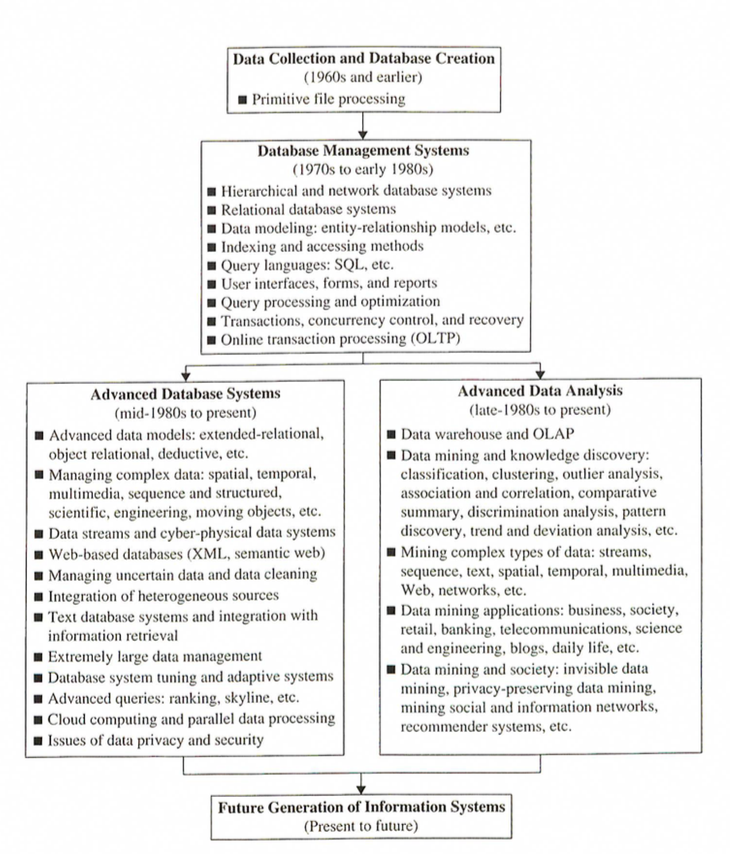
\includegraphics[width=0.6\textwidth]{images/dbevolution}
	\caption{Entwicklung von Datenbank Technologien \cite{DataMiningConceptsAndTechniques}}
	\label{fig:dbevolution}
\end{figure}

Der Term \textit{data mining} ist eigentlich nicht beschreibend, da dieser nur ein Teil des \textit{knowledge discovery process} ist. Im allgemeinem besteht der Knowledge Discovery Prozess aus den folgenden iterierenden Schritten.

\begin{enumerate}
\item \textbf{Daten Reinigung} wo inkonsistente Daten verworfen werden
\item \textbf{Daten Integration} wo mehrere Datenquellen zu einer vereinigt werden
\item \textbf{Daten Selektion} wo Daten, welche für die analyse relevant sind, von einer Datenbank geholt werden
\item \textbf{Data Mining} wo Algorithmen angewandt werden um Datenmuster zu erkennen
\item \textbf{Musterevaluierung} wo die \textit{interessanten} Muster endgültig identifiziert werden.
\item \textbf{Präsentation} wo die Daten für User dargestellt werden.
\end{enumerate}

Diese Schritte können im allgemeinem für jede Art an Daten angewandt werden, so lang wie diese auch für die Applikation relevant sind. Die einfachsten Arten von Datamining Applikationen sind Datenbank Daten, Data Warehouse Daten, und Daten die bei Transaktionen entstehen. Es besteht aber auch die Möglichkeit Data Mining bei anderen Arten von Daten durchzuführen, z.B. Datenstreams, Sequenzielle Daten, Graph oder Netzwerk Daten, Text Daten, Multimedia Daten und das WWW. 

\subsection{Datenbank Daten}
Ein Datenbanksystem, auch als Datenbankmanagementsystem (DBMS) bekannt, besteht aus einer Ansammlung an zusammenhängenden Daten und Software, welche den Zugriff und die Verwaltung dieser ermöglichen. Diese Software stellt Mechanismen zur Verfügung, welche für die Definition einer Struktur der Daten, für die Einhaltung von Konsistenz, für die Sicherheit der Daten selbst bei unerwarteten Abstürzen des Systems, verwendet werden

Grundsätzlich werden bei so genannten relationalen Datenbanken die Daten in Tabellen eingeordnet. Die Tabelle besteht aus Attributen \textit{(columns oder fields)} und speichert normalerweise eine große Anzahl an Tupeln \textit{(records and rows)}. Jede dieser Einträge in der Tabelle ist eindeutig identifizierbar durch einen so genannten \textit{unique key}. Ein semantisches Model, wie ein \textit{entity-relationship (ER)} Model, werden oft erstellt um die Daten und deren Beziehungen in Tabellenform darzustellen.

Der Zugriff auf die relationalen Daten erfolgt mittels Datenbank Queries, welche in einer relationalen Abfragsprache (z.B. SQL) oder mittels einem graphischem Interface geschrieben werden. Diese Abfragen ermöglichen es spezifische Daten aus einer enormen Anzahl zu erhalten. Eine beispielhafte Anfrage an das DBMS ist \textit{„Zeige mir eine Liste von allen Dingen, die im letzten Quartal verkauft wurden“} oder mittels den integrierten Aggregatfunktionen \textit{„Welcher Verkäufer hatte die größte Anzahl an Empfelungen“}.

Mittels Datamining und den Daten der relationalen Datenbank kann mehr aus den Daten herausgeholt werden, wie aktuelle Trends oder gewisse Muster. Zum Beispiel ist es möglich das Kaufmuster einer Person zu erkennen um die Kreditwürdigkeit basierend auf Alter, Gehalt und bisherige Kredite zu prognostizieren.

\subsection{Data Warehouses}
W.H. Inmon beschreibt ein Data-Warehouse als Ansammlung verschiedener Information aus vielen unterschiedlichen Quellen, diese sind dann in einer dafür spezifizierten Datenbank gespeichert \cite{DataWarehouseAAG}. Auch hier werden die Daten zuerst gesäubert, dann in die Datenbank integriert, transformiert, geladen und periodisch erneuert. Die Daten werden auch in verschiedene große Kategorien geschlichtet. Es werden aber nicht alle Daten gespeichert, nur jene, die das Objekt am besten beschreiben \cite{DataMiningConceptsAndTechniques}. 

Ein Data Warehouse ist normalerweise in einer multidimensionalen Daten Struktur der \textit{Data Cube} gennant. Bei diesem Data Cube ist jede Dimension ein oder mehrere Attribute, jede Zelle speichert den Wert einer Aggregat Funktion der Daten (d.h. vereinfachte Daten). 

In Abbildung \ref{fig:dbwarehouse} kann der typischer Aufbau eines Data Warehouses gesehen werden. In dieser werden auch die benötigten Schritte veranschaulicht.

\begin{figure}[!h]\centering
	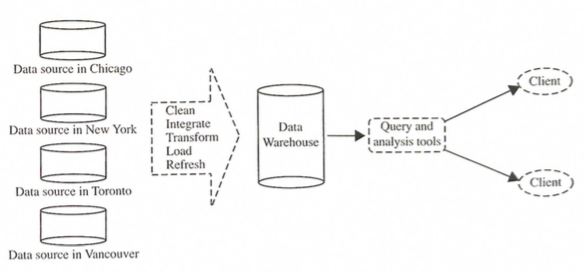
\includegraphics[width=0.8\textwidth]{images/dbwarehouse}
	\caption{Beispielhafter Aufbau eines Data Warehouses\cite{DataMiningConceptsAndTechniques}}
	\label{fig:dbwarehouse}
\end{figure}


\subsection{Daten von Transaktionen}

\subsection{Verwendete Technologien}

\subsubsection{Statistiken}

\subsubsection{Machine Learning}

\subsubsection{Datenbank Systeme und Data Warehouses}

\subsubsection{Informationsbeschaffung}
